\section{Análise exploratória}\label{sec:sv_eda}

\svPositivos\% das pessoas ganham mais de 50 mil, cerca de \svRazaoClasses{} pessoas abaixo para cada uma acima: responder sempre ``até 50 mil'' já acerta \svPiso\%, e esse é o piso. Entre os numéricos, os anos de estudo têm a maior correlação com o rótulo (\svCorrEstudo), seguidos da idade (\svCorrIdade), das horas por semana (\svCorrHoras), do ganho de capital (\svCorrGanho) e da perda de capital (\svCorrPerda). Entre os categóricos, o estado civil é o que mais separa: entre os casados, \svCasados\% ganham mais de 50 mil; entre quem nunca casou, \svNuncaCasou\% (Figura~\ref{fig:sv_eda}a). A renda alta cresce com os anos de estudo: \svEstudoNove\% com 9 anos, \svEstudoTreze\% com 13 e \svEstudoQuinze\% com 15 (Figura~\ref{fig:sv_eda}b).

\begin{figure}[ht]
\centering
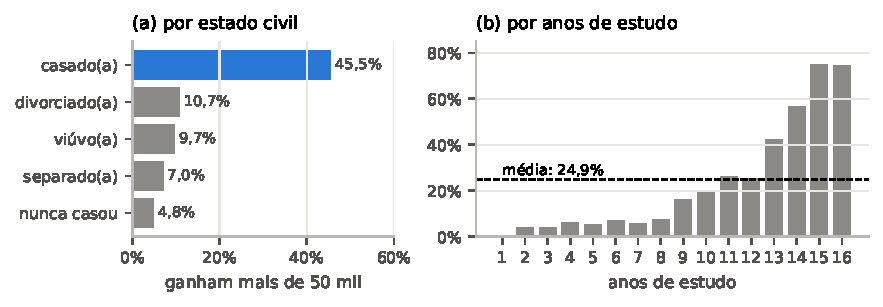
\includegraphics[width=\textwidth]{figures/svm_eda.pdf}
\caption{Proporção de pessoas que ganham mais de 50 mil (a) por estado civil, nas cinco categorias mais comuns, e (b) por anos de estudo, na base inteira (\svLinhas{} pessoas). A linha tracejada é a proporção geral.}
\label{fig:sv_eda}
\end{figure}


Mesmo o atributo mais forte não basta: nem entre os casados a renda alta passa da metade. Separar as classes exige, portanto, combinar vários atributos, e a distância entre o piso (\svPiso\%) e o teto (\svTeto\%) é o espaço em que os modelos competem.
